\documentclass[a4paper]{article}
\usepackage{tikz}
\usetikzlibrary{trees}

%% Language and font encodings
\usepackage[english]{babel}
\usepackage[utf8x]{inputenc}
\usepackage[T1]{fontenc}

%% Sets page size and margins
\usepackage[a4paper,top=3cm,bottom=2cm,left=3cm,right=3cm,marginparwidth=1.75cm]{geometry}

%% Useful packages
\usepackage{amsmath}
\usepackage{graphicx}
\usepackage[colorinlistoftodos]{todonotes}
\usepackage[colorlinks=true, allcolors=blue]{hyperref}

\title{Mini Assignment 0}
\author{Derrick Heinemann}

\begin{document}
\maketitle

Given the following grammar:\\

$<$VarDecl$>$ $\rightarrow$ int $<$VarList$>$ ;

$<$VarList$>$ $\rightarrow$ $<$Identifier$>$ $\mid$

$<$Identifier$>$ , $<$VarList$>$ $\mid$

$<$Identifier$>$ $\rightarrow$ $<$Letter$>$ $\mid$ $<$Identifier$>$ $<$Letter$>$ $\mid$ $<$Identifier$>$ $<$Digit$>$

$<$Integer$>$ $\rightarrow$ $<$Digit$>$ $\mid$ $<$Digit$>$ $<$Integer$>$ 

$<$Letter$>$ $\rightarrow$ a $\mid$ b $\mid$ c $\mid$ d

$<$Digit$>$ $\rightarrow$ 1 $\mid$ 2 $\mid$ 3 $\mid$ 4\\

Provide a parse tree showing that:

int a, b, c; 

is a valid $<$VarDecl$>$. \\ \\

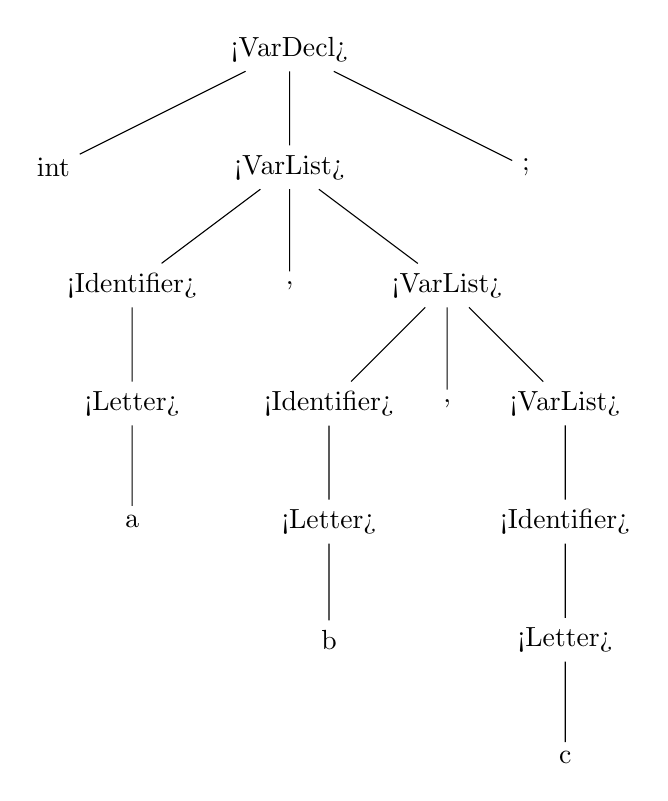
\begin{tikzpicture}[level distance=1.5cm,
  level 1/.style={sibling distance=3cm},
  level 2/.style={sibling distance=2cm},
  level 3/.style={sibling distance=1.5cm}]
  \node {<VarDecl>}
    child {node {int}}
    child {node {<VarList>}
    	child {node {<Identifier>}
        	child {node {<Letter>}
            	child {node {a}}}}
        child {node {,}}
        child {node {<VarList>}
        	child {node {<Identifier>}
            	child {node {<Letter>}
                	child {node {b}}}}
            child {node {,}}
            child {node {<VarList>}
            	child {node {<Identifier>}
                	child {node {<Letter>}
                    	child {node {c}}}}}}
        }
    child {node {;}};
\end{tikzpicture}

\end{document}